\documentclass[conference]{IEEEtran}
\IEEEoverridecommandlockouts
\usepackage{cite}
\usepackage{amsmath,amssymb,amsfonts}
\usepackage{graphicx}
\usepackage{textcomp}
\usepackage{xcolor}
\usepackage{booktabs}
\usepackage{multirow}
\usepackage{url}
\newcommand{\todo}[1]{\textcolor{red}{[#1]}}
\graphicspath{{../figures/}{./}}

\begin{document}
\bstctlcite{IEEEexample:BSTcontrol}

\title{Deep Reinforcement Learning for Power-Limited Electric Vehicle Charging Hubs with Leave-One-Site-Out Evaluation on Four Public Session Datasets}

\author{\IEEEauthorblockN{Gabrielly de Queiroz Pereira\IEEEauthorrefmark{1},
Amanda Aparecida Stadler\IEEEauthorrefmark{3},
Marcella Scoczynski Ribeiro Martins\IEEEauthorrefmark{2}\IEEEauthorrefmark{3},\\
Jonathan de Matos\IEEEauthorrefmark{1},
Zito Palhano da Fonseca\IEEEauthorrefmark{1} and
Maria Salete Marcon Gomes Vaz\IEEEauthorrefmark{1}}
\IEEEauthorblockA{\IEEEauthorrefmark{1}Department of Informatics, Graduate Program in Applied Computing, State University of Ponta Grossa (UEPG), Brazil\\
\IEEEauthorrefmark{2}Academic Department of Electronics, \IEEEauthorrefmark{3}Graduate Program in Electrical Engineering, UTFPR, Ponta Grossa, Brazil\\
{\small gqpereira@uepg.br, amandaastadler@gmail.com, marcella@utfpr.edu.br, jonathan@uepg.br, zpfonseca@uepg.br, salete@uepg.br}}}

\maketitle

\begin{abstract}
Deep reinforcement learning (DRL) controllers for electric-vehicle charging are usually trained and
evaluated on data from a single site. This paper evaluates a proximal policy optimization (PPO)
controller for a charging hub with a shared power limit at sites excluded from training, using
280\,022 public AC sessions from four datasets (Palo Alto, Dundee, Perth and Kinross, Trondheim) and
GB half-hourly prices in weekly episodes with chronological splits. The controller outputs a hub
set-point that a safety layer allocates by least laxity; flat, DeepSets and self-attention state
encoders were compared after tuning with Optuna. In leave-one-site-out tests with five seeds, the PPO agents had a mean regret with respect to
the clairvoyant optimum of 7.1--7.5\%, against 7.6\% for least-laxity-first (LLF) and 3.6\% for a
receding-horizon linear program (MPC). With a 1\,h error in the announced departures, the regret of MPC
rose to 21.6\%, that of PPO to 10.9--11.9\% and that of LLF to 8.9\%. Pooling three source sites did
not reduce the regret at the held-out site with respect to the best single source.
\end{abstract}

\begin{IEEEkeywords}
electric vehicles, smart charging, deep reinforcement learning, zero-shot generalization, set neural networks, smart grids
\end{IEEEkeywords}

%=========================================================================================
\section{Introduction}
%=========================================================================================
Uncoordinated charging of plug-in vehicles on a local scale can lead to grid problems, analysed
in terms of power losses and voltage deviations, and coordinated charging was proposed to reduce
them~\cite{clement2010impact}. As the fleet grows, an intelligent charging management system is
expected to be necessary to limit network reinforcement costs, voltage deviations and transformer
saturation~\cite{garcia2014review}. The time at which charging is shifted also matters for the
equipment: simulations of a 25\,kVA distribution transformer showed that temperature-based smart
charging reduced the mean and variance of transformer aging, while delaying charging until after
midnight could increase aging~\cite{hilshey2013transformer}.

Optimization-based scheduling is already operated at scale: the Adaptive Charging Network uses an
algorithm based on convex optimization and model predictive control and has been deployed at more
than one hundred sites~\cite{lee2021acn}. Such schedulers consume the departure time and energy
announced by each driver~\cite{lee2021acn}, and the analysis of the public ACN-Data set found that
these user inputs are unreliable and gave the worst prediction among the compared
estimators~\cite{lee2019acndata}.

Deep reinforcement learning (DRL) has been proposed as an alternative that formulates charging
as a Markov decision process with unknown transition probabilities and learns a policy without a
model of the system~\cite{wan2019modelfree}. Continuous-action DRL has been applied to the
charging of an individual vehicle under dynamic user behaviour and prices~\cite{yan2021sac}, and
a review of DRL-based charging management lists the uncertainty of vehicle parameters, energy
prices and loads as the main difficulty addressed by these methods~\cite{abdullah2021review}.
Open simulators support this line of work: ACN-Sim replays ACN-Data sessions and exposes an
OpenAI Gym interface~\cite{lee2021acnsim}, and the EV2Gym authors report that only a few smart
charging simulators provide a Gym environment for RL~\cite{orfanoudakis2025ev2gym}.

Three limitations motivate this study. First, a DRL policy that is deployed at a new site faces a
problem of zero-shot generalization, in which a policy must perform in situations not seen in
training instead of overfitting to its training environment~\cite{kirk2023survey}; for charging,
Li and Sun describe MPC as conservative and data-independent and RL as fully trusting its data, and
evaluate an OOD-aware scheduler under the change in charging behaviour that COVID-19 caused in
ACN-Data~\cite{li2023ood}. Second, public session data come from different populations, such as a
workplace campus~\cite{lee2019acndata} and residential apartment buildings~\cite{sorensen2021data},
whose flexibility depends on parking and charger arrangements~\cite{sorensen2021flex}. Third,
DRL results vary with seeds and implementation details, so comparisons without repeated runs and
significance tests are hard to interpret~\cite{henderson2018matters}.

The objective of this paper is to measure, on four public session datasets from three countries,
how a DRL controller for a charging hub with a shared power limit performs at a site that was
excluded from training, and how this performance compares with heuristic, optimization-based and
clairvoyant references when the announced departure times contain errors. The contributions are:
(i) a harmonized benchmark of 280\,022 public AC charging sessions with real half-hourly prices and
temporally disjoint train, validation and test periods, replayed in a simulator checked against
ACN-Sim~\cite{lee2021acnsim}; (ii) a PPO controller with a permutation-invariant encoder over the
plugged-in vehicles and a one-dimensional set-point action that applies to hubs of any size;
(iii) a leave-one-site-out evaluation with five seeds, paired statistical tests and ablations of
the training design. The study addresses the ICIT topics of adaptive and intelligent control
systems, machine learning, and transportation systems: the hubs considered share an electrical
infrastructure that can be over-subscribed~\cite{lee2021acn} and charge under time-varying
prices~\cite{wan2019modelfree}.

%=========================================================================================
\section{Data and Simulation Environment}
%=========================================================================================
Fig.~\ref{fig:flow} summarizes the pipeline.

\begin{figure}[t]
\centering
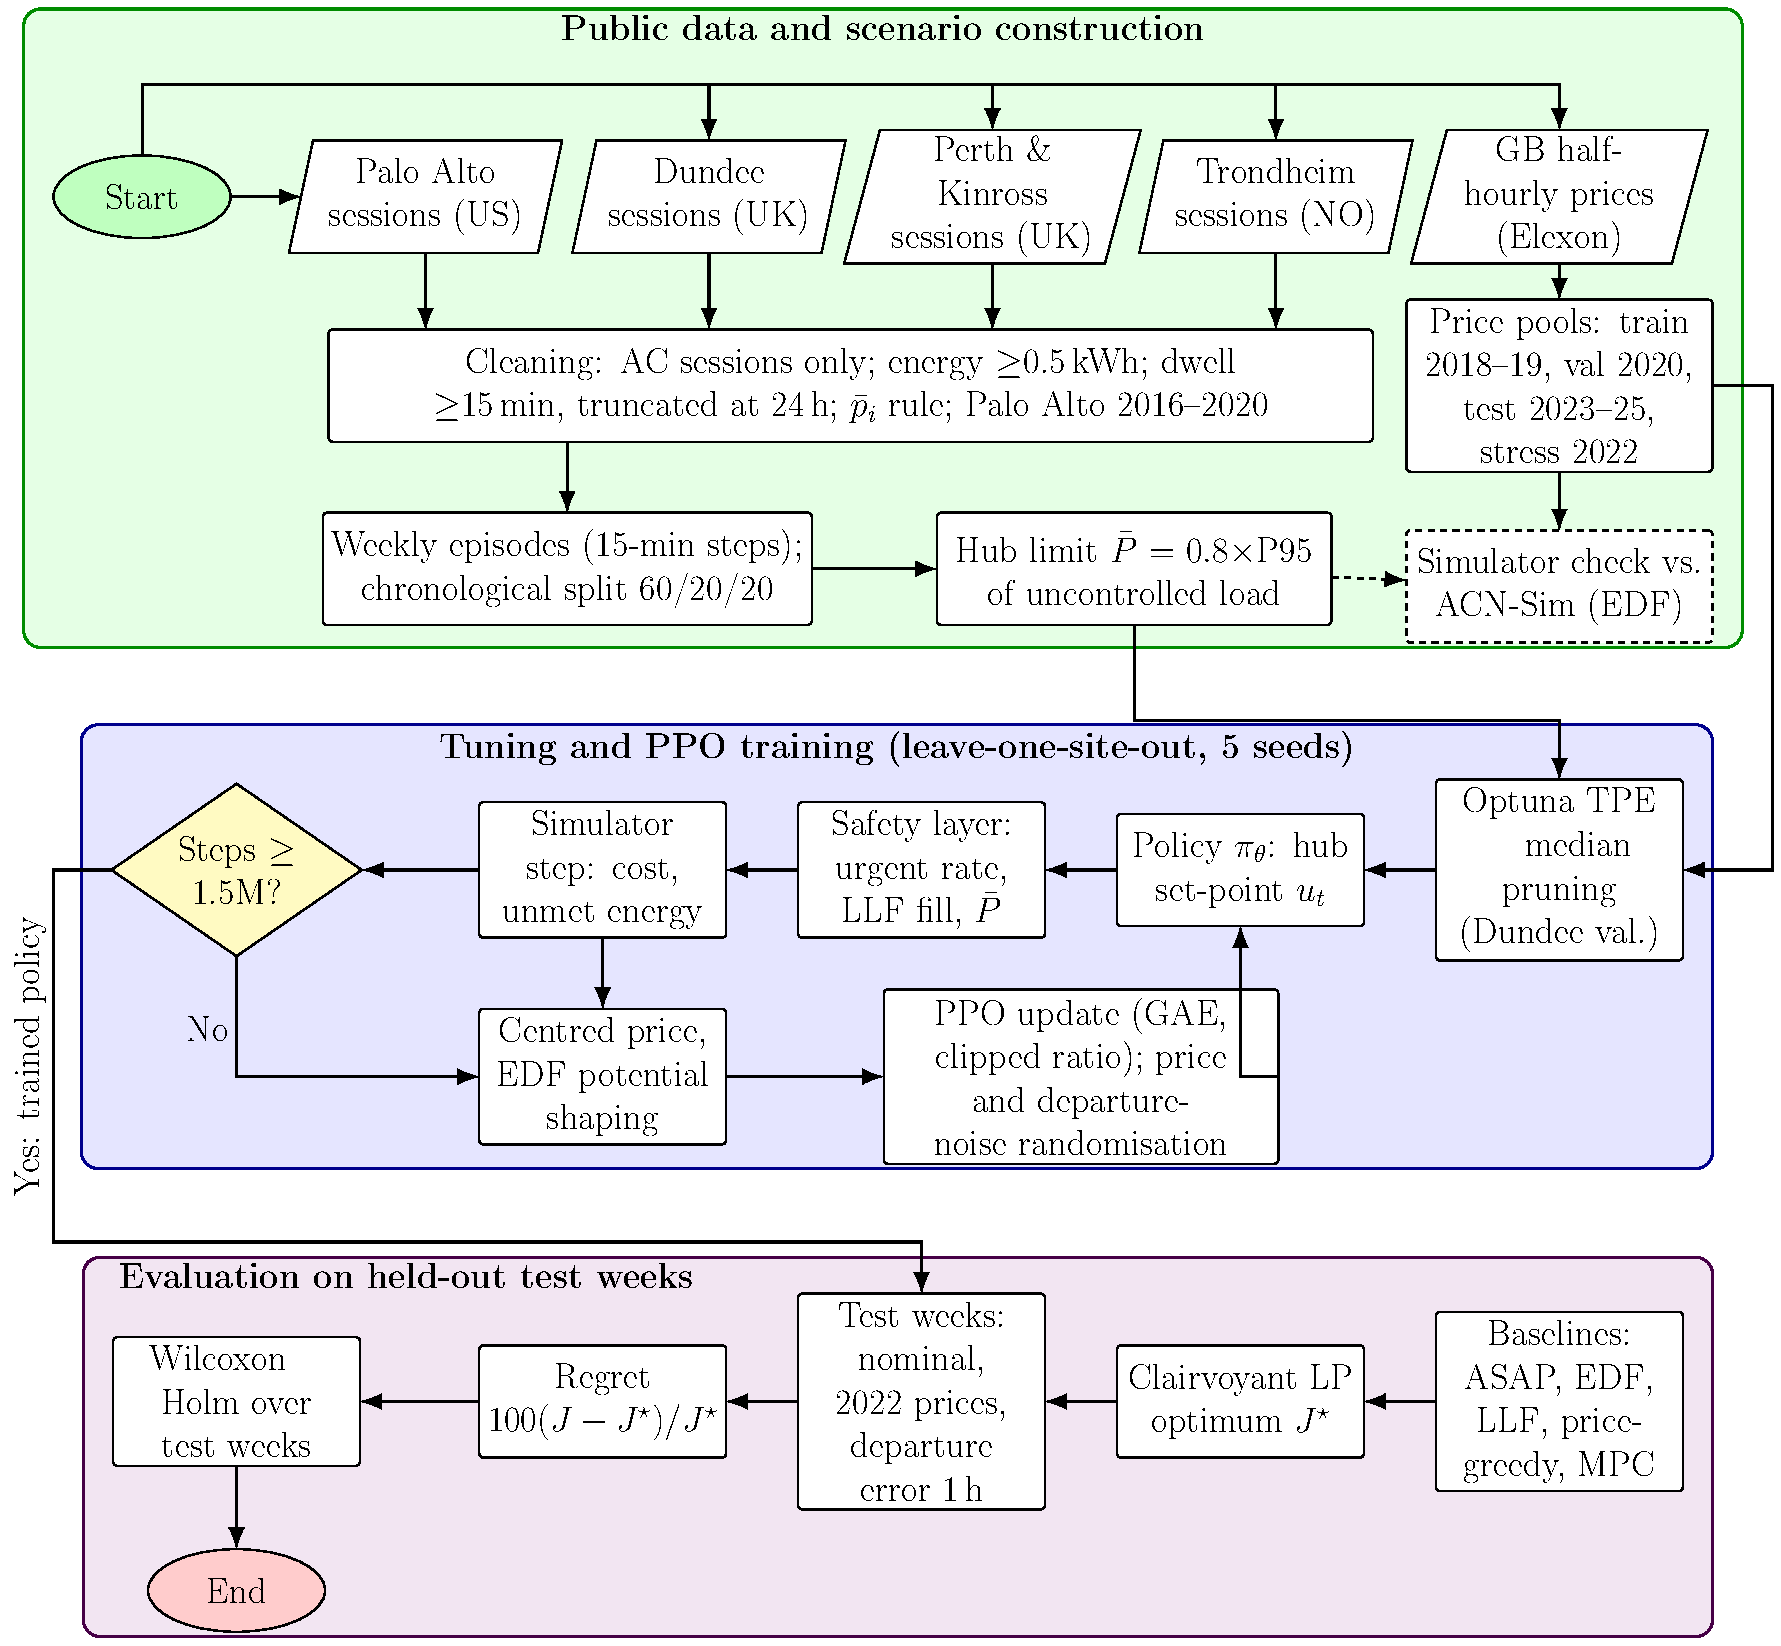
\includegraphics[width=\columnwidth]{fig_flowchart.pdf}
\caption{Pipeline of the study: public data and scenario construction, hyperparameter tuning and
PPO training with leave-one-site-out sources, and evaluation on held-out test weeks.}
\label{fig:flow}
\end{figure}

\subsection{Session datasets and cleaning}
Four public datasets were used (Table~\ref{tab:data}): the City of Palo Alto public charging
network~\cite{paloalto}, the Dundee City Council public network~\cite{dundee}, the Perth and Kinross
Council network~\cite{perth}, and charging reports from Norwegian apartment
buildings~\cite{sorensen2021data}. Each record was mapped to arrival time, departure (plug-out)
time, delivered energy and charger identifier. Table~\ref{tab:data} lists the cleaning rules and the
sessions removed by each. Palo Alto sessions before 2016 were removed because the network was being
built out, the two Dundee 2024 files overlap, and DC
rapid sessions leave no room for shifting.
The maximum rate of session $i$ is $\bar p_i=\min(\max(p^{\mathrm{nom}},1.1E_i/w_i),22)$\,kW, where
$w_i$ is the dwell time and $p^{\mathrm{nom}}$ is 6.6\,kW for Palo Alto Level~2 (1.9\,kW Level~1),
7.4\,kW for Dundee and Perth and 3.7\,kW for Trondheim; the observed average rate is a lower bound of
the vehicle rate. The requested energy $E_i$ is the delivered energy, capped at $0.98\,\bar p_i w_i$.

\begin{table}[t]
\caption{Sessions removed per cleaning rule, statistics after cleaning (idle share
$1-E_i/(\bar p_i w_i)$) and weekly episodes per split.}
\label{tab:data}
\centering
\footnotesize
\setlength{\tabcolsep}{1.5pt}
\begin{tabular}{lrrrr}
\toprule
 & Palo Alto & Dundee & Perth & Trondheim\\
 & (US, public) & (UK, public) & (UK, public) & (NO, resid.)\\
\midrule
Raw records & 259\,415 & 501\,450 & 66\,664 & 6\,878\\
Before 2016 & $-$52\,818 & -- & -- & --\\
Duplicates & -- & $-$110\,957 & $-$7 & --\\
DC / rapid models & -- & $-$321\,514 & $-$51\,435 & --\\
Unparseable fields & 0 & $-$1\,941 & $-$58 & $-$34\\
Dwell $<$ 15 min & $-$8\,068 & $-$4\,167 & $-$1\,652 & $-$173\\
Energy $<$ 0.5 kWh & $-$805 & $-$511 & $-$231 & $-$14\\
\textbf{Sessions kept} & \textbf{197\,724} & \textbf{62\,360} & \textbf{13\,281} & \textbf{6\,657}\\
Dwell cut to 24 h & 22 & 2\,457 & 459 & 456\\
\midrule
Period & 2016--20 & 2021--25 & 2016--19 & 2018--20\\
Chargers & 80 & 67 & 40 & 110\\
Mean energy (kWh) & 9.2 & 16.4 & 11.0 & 13.1\\
Mean dwell (h) & 2.6 & 5.8 & 4.4 & 10.2\\
Mean idle share (\%) & 40 & 42 & 52 & 51\\
\midrule
Weeks train/val./test & 157/52/53 & 128/43/43 & 101/35/35 & 32/12/12\\
Med. $\bar P$ tr./test (kW) & 80.2/40.3 & 56.7/53.1 & 18.0/30.9 & 13.5/39.9\\
Test weeks from & 2019-12 & 2024-11 & 2019-02 & 2019-11\\
\bottomrule
\end{tabular}
\end{table}

\subsection{Prices}
Half-hourly GB market index prices (APX) for 2018--2025 were downloaded from the Elexon Insights
API~\cite{elexon}; auctions with zero volume were treated as missing and interpolated, and the
series was resampled to 15\,min. The same price signal is used at every site so that differences
between sites come from user behaviour and hub size. Price weeks are split into disjoint pools:
training 2018--2019 (105 weeks), validation 2020 (52), test 2023--2025 (137) and a stress pool
with the 2022 energy-crisis prices (52). Within an episode, prices are divided by their mean over
the episode, and the controller sees the day-ahead prices of the next 24\,h.

\subsection{Episodes and hub limit}
An episode is one calendar week of real arrivals (Monday 00:00 to Monday 00:00) followed by a 24\,h
tail, discretized in $\Delta=15$\,min steps (768 steps). Arrival steps are rounded up and departure
steps down, with at least one step of dwell. Weeks with fewer than 10 sessions are discarded
(3 weeks at Perth and Trondheim). The weeks of each site are split chronologically into 60\% training,
20\% validation and 20\% test, so that test weeks are later than all training weeks
(Table~\ref{tab:data}). Week $k$ of a split is paired with price week $k \bmod N$ of the
corresponding pool; the pairing is fixed and identical for all methods. Each dataset is treated as
one virtual hub: the sessions of all its chargers share one power limit, which represents an aggregator
or a common feeder and not the physical layout of the network. The hub has $M=48$ charger
slots (the largest observed concurrency is 45; no session was lost to a full hub). Because the
networks grew over the years, the hub limit $\bar P$ is set per week to $0.8$ times the 95th percentile of the load that the week
produces under uncontrolled charging, with a floor equal to the largest $\bar p_i$ of the week.

\subsection{Objective and reference optimum}
With rates $r_{i,t}\in[0,\bar p_i]$ while vehicle $i$ is plugged in and
$\sum_i r_{i,t}\le\bar P$, the weekly objective is
\begin{equation}
J=\sum_{t}p_t\,\Delta\sum_i r_{i,t}+\lambda\sum_i u_i,\qquad
u_i=E_i-\Delta\!\!\sum_{t<d_i}r_{i,t},
\label{eq:J}
\end{equation}
with normalized price $p_t$, undelivered energy $u_i\ge0$ and $\lambda=3$ (three times the mean
price of the week). The clairvoyant optimum $J^\star$, which knows all arrivals, departures and
energies of the week, is the linear program \eqref{eq:J} solved with the HiGHS solver
through SciPy. Results are reported as regret $100(J-J^\star)/J^\star$ (\%), together with the
fraction of requested energy delivered and the energy cost per delivered kWh.

\subsection{Simulator and its check against ACN-Sim}
The simulator is vectorized in NumPy over a batch of episodes. A new vehicle occupies the lowest
free slot; at every step, rates are clipped to $\bar p_i$ and to the remaining energy and the hub
limit is enforced (Section~\ref{sec:safety}). To check the implementation, five validation weeks
per site were replayed with earliest-deadline-first (EDF) scheduling in this simulator and in
ACN-Sim~\cite{lee2021acnsim} (acnportal 0.3.3), using a 1000\,V single-phase network (1\,A = 1\,kW),
ideal batteries and a common maximum rate of 7\,kW, since the EDF of ACN-Sim allocates up to the
charger limit and not up to the vehicle limit. The difference in delivered energy, relative to
demand, was between $-0.26\%$ and $+0.12\%$ over the 20 weeks (\texttt{scripts/validate\_acnportal.py}).

%=========================================================================================
\section{Controller and Training}
%=========================================================================================
\subsection{Action and safety layer}\label{sec:safety}
A policy with one Beta-distributed action per slot (48 dimensions) is retained as an ablation. Since all vehicles
pay the same price at a given step, the choice of \emph{which} vehicle charges only affects the
deadlines. The policy therefore outputs one hub set-point $u_t\in[0,1]$, held for $k$ simulator
steps. A safety layer converts it into rates in two passes ordered by least laxity
(laxity = announced time left minus time needed at $\bar p_i$): first, each vehicle receives the
\emph{urgent} rate
$\underline r_{i,t}=[(e_{i,t}-\bar p_i(\hat d_i-t-1)\Delta)/\Delta]^+$, the smallest rate that still
allows completion at full power, up to $\bar P$; second, the remainder of $u_t\bar P$ is distributed,
again by least laxity, up to each vehicle's feasible rate. The hub limit is never exceeded.

\subsection{State and policy network}
Each occupied slot is described by six features: presence, energy still needed expressed in days at
$\bar p_i$, announced time left (days), laxity (days), $\bar p_i/22$ and remaining fraction of
$E_i$. Global features (33 values) are sine and cosine of hour and weekday, occupancy, feasible
power over $\bar P$, current price as z-score and rank within the next 24\,h, the 24 hourly
z-scores of the next day, elapsed fraction of the episode, urgent power over $\bar P$, the maximum
deficit of the EDF demand condition (below) normalized by one day of $\bar P$, and pending energy
normalized by one day of $\bar P$. Three encoders were compared: (a) a flat MLP over the 48
zero-padded slots and the global features; (b) DeepSets~\cite{zaheer2017deepsets}: a shared MLP
$\phi$ embeds each slot concatenated with the global features, followed by masked mean and max
pooling; (c) the same encoder with one multi-head self-attention layer and layer normalization
before pooling~\cite{vaswani2017attention}. Actor and critic are one-hidden-layer heads on the
pooled vector and the global features; the actor outputs the parameters $\alpha=1+\mathrm{softplus}(\cdot)$
and $\beta=1+\mathrm{softplus}(\cdot)$ of a Beta distribution for $u_t$, initialized with mean 0.6.
Evaluation uses the mean of the Beta distribution. Encoders (b) and (c) are permutation invariant
and do not depend on $M$.

\subsection{Learning signal}
\emph{Centred price.} Since $\Delta\sum_{t,i}r_{i,t}=D-U$, with $D=\sum_iE_i$ exogenous and
$U=\sum_iu_i$, \eqref{eq:J} equals $\sum_t(p_t-1)\Delta\sum_ir_{i,t}+(\lambda-1)U+D$. Training on
the first two terms changes the reward of each step but not the optimal policy.
\emph{Shaping.} The potential
$\Phi(s)=-(\lambda-1)\max\!\big(\sum_i[e_i-\bar p_i\tau_i\Delta]^+,\ \max_k[\sum_{\hat d_i\le\hat d_k}e_i-\bar P\tau_k\Delta]^+\big)$,
with $\tau$ the announced steps left, is a lower bound on the energy of the plugged-in vehicles that
can no longer be delivered (the second term is the EDF demand condition for the shared limit). The
shaping term $\gamma\Phi(s')-\Phi(s)$ preserves the optimal policies~\cite{ng1999shaping}.
\emph{Normalization.} Global features are normalized with running mean and standard deviation
(clipped to $\pm10$) and rewards are divided by the running standard deviation of the discounted
return. \emph{Augmentation.} In the final runs, each sampled training week is paired with a random
week of the training price pool, and the announced departure of each vehicle is perturbed by
$\mathcal N(0,\sigma^2)$, with $\sigma\sim U[0,1.5]$\,h drawn per batch of episodes (domain
randomization~\cite{tobin2017domain}).

\subsection{PPO, tuning and seeds}
PPO~\cite{schulman2017ppo} with generalized advantage estimation, Adam ($\epsilon=10^{-5}$),
gradient-norm clipping 0.5, value coefficient 0.5, 8 minibatches per epoch and linear decay of the
learning rate was used. Hyperparameters were tuned with Optuna (TPE sampler, median pruner at half
of the budget)~\cite{akiba2019optuna} on the Dundee training weeks, scored on 20 Dundee validation
weeks, with $10^6$ simulator steps per trial and without augmentation (Table~\ref{tab:hpo}). The
DeepSets study ran 10 trials (7 completed, 3 pruned) and the MLP study 20 trials (13 completed,
7 pruned). The first attention trial had not finished after 1.6\,h (DeepSets: 14--76\,min), so the
attention encoder was not tuned and reuses
the DeepSets configuration with four heads. Final agents were trained for $1.5\times10^6$ simulator steps with 16 parallel weeks.

\begin{table}[t]
\caption{Search space and selected hyperparameters.}
\label{tab:hpo}
\centering
\footnotesize
\setlength{\tabcolsep}{3pt}
\begin{tabular}{lll l}
\toprule
Parameter & Search space & DeepSets & MLP\\
\midrule
Hidden width & \{64, 128, 256\} & 64 & 128\\
Layers of $\phi$ / body & \{1, 2, 3\} & 2 & 1\\
Activation & \{tanh, ReLU\} & tanh & tanh\\
Learning rate & $[10^{-4},10^{-3}]$ log & $1.17\times10^{-4}$ & $1.43\times10^{-4}$\\
Entropy coef. & $[10^{-5},10^{-2}]$ log & $9.7\times10^{-3}$ & $2.0\times10^{-3}$\\
$\gamma$ (per decision) & \{0.95, 0.97, 0.99\} & 0.97 & 0.95\\
GAE $\lambda$ & \{0.90, 0.95, 0.98\} & 0.90 & 0.98\\
Clip ratio & \{0.1, 0.2, 0.3\} & 0.2 & 0.1\\
Epochs & \{3, 5, 10\} & 10 & 10\\
Rollout length & \{48, 96, 192\} & 192 & 48\\
Decision interval $k$ & \{2, 4\} steps & 2 (30 min) & 2 (30 min)\\
Parallel weeks & \{16, 32\} & 16 & 16\\
\midrule
Validation $J$/kWh & & 0.9666 & 0.9697\\
\bottomrule
\end{tabular}
\end{table}

Seeds control the PyTorch initialization and sampling, NumPy, the sampling of training weeks,
price weeks and departure noise (through a seeded generator), and the departure noise of the test
conditions. Two runs with the same seed produced identical training rewards and test costs to the
eighth decimal on the same machine. All runs used an Intel Core i7-1355U CPU (10 cores, 16\,GB RAM,
no GPU), Python 3.10, PyTorch 2.10, NumPy 1.26.4, SciPy 1.15.3, pandas 2.3.3 and Optuna 5.0.0.

%=========================================================================================
\section{Experimental Protocol}
%=========================================================================================
\emph{Baselines.} ASAP charges every vehicle at its maximum rate and scales all rates proportionally
when $\bar P$ is exceeded (uncontrolled charging). EDF and LLF fill $\bar P$ in order of earliest
announced departure and of least laxity. Price-greedy books, at arrival, the cheapest known
15-min steps of each vehicle's window and charges at full power when the laxity reaches one step.
MPC solves, at each arrival and at least every hour, the linear program \eqref{eq:J} restricted to
the vehicles plugged in, with day-ahead prices up to their announced departures, and applies the
first step; it has no forecast of future arrivals. It simplifies the convex-optimization MPC of the ACN~\cite{lee2021acn}. The +S variants apply the same safety layer as
the PPO agent.

\emph{Experiments.} E2 (leave-one-site-out): an agent is trained on the training weeks of three sites
and tested on the test weeks of the fourth, for each encoder and five seeds (DeepSets and MLP) or
three seeds (attention). E1 (single source): an agent trained on one site is tested on all four
(two seeds, DeepSets and MLP). E3 (ablations, one seed, leave-one-site-out): no shaping, no centred
price, per-slot actions, and no departure noise in training.

\emph{Test conditions.} Nominal (test weeks with 2023--2025 prices), stress (same weeks with 2022
prices) and departure error (nominal, with the announced departure of every vehicle perturbed by
$\mathcal N(0,1\,\mathrm h)$, seeded identically for all methods). The clairvoyant optimum uses the
true departures.

\emph{Statistics.} For each held-out site, regrets are averaged over seeds per test week and
compared between methods with the two-sided Wilcoxon signed-rank test over weeks; $p$-values are
adjusted with the Holm procedure over the four sites of each comparison.

%=========================================================================================
\section{Results}
%=========================================================================================
\subsection{Held-out sites (E2)}
Table~\ref{tab:main} lists the regret on the test weeks of each held-out site and Fig.~\ref{fig:regret}
shows its distribution over weeks. Under nominal conditions, MPC with the safety layer had the lowest
mean regret at Dundee (3.8\%), Perth (3.4\%) and Trondheim (1.1\%), and LLF the lowest at Palo Alto
(2.5\%). The three PPO encoders, trained without the held-out site, reached 7.1--7.5\% averaged over
the four sites (standard deviation over seeds 0.2--0.3 points), against 7.6\% for LLF, 6.4\% for
price-greedy+S and 3.6\% for MPC+S. Per site, PPO had a lower regret than LLF at Dundee, Perth and
Trondheim (Holm-adjusted $p<0.003$ for the three encoders) and a higher regret at Palo Alto, where
PPO-MLP (3.1\%) was also below MPC+S (4.2\%, $p_\mathrm{Holm}<0.001$). With the 2022 crisis prices, the regrets changed by at most 2.3 points and the method with the lowest
regret at each site was the same as under nominal prices. ASAP had its largest regret at Trondheim
(20.5\%), the residential site with a mean dwell of 10.2\,h (Table~\ref{tab:data}), where S{\o}rensen et al. reported a
flexibility potential for apartment buildings with private charge points~\cite{sorensen2021flex}.

\begin{table}[t]
\caption{Regret (\%) on the test weeks of each held-out site (E2). PPO: mean $\pm$ standard
deviation over seeds (5 seeds; attention 3 seeds). ASAP does not use departures and is unchanged
under departure error.}
\label{tab:main}
\centering
\footnotesize
\setlength{\tabcolsep}{2.2pt}
\begin{tabular}{llcccc}
\toprule
 & Method & Palo Alto & Dundee & Perth & Trondheim\\
\midrule
\multirow{7}{*}{\rotatebox{90}{Nominal}}
& ASAP & 5.9 & 18.5 & 11.6 & 20.5\\
& LLF & 2.5 & 12.8 & 6.4 & 15.2\\
& Price-greedy+S & 4.8 & 8.0 & 6.3 & 8.0\\
& MPC+S & 4.2 & 3.8 & 3.4 & 1.1\\
& PPO-MLP & 3.1$\pm$0.2 & 11.9$\pm$0.6 & 5.6$\pm$0.5 & 12.4$\pm$2.4\\
& PPO-DeepSets & 4.3$\pm$0.3 & 11.7$\pm$0.7 & 5.9$\pm$0.1 & 11.3$\pm$1.7\\
& PPO-Attention & 4.3$\pm$0.2 & 10.8$\pm$0.8 & 6.0$\pm$0.2 & 10.8$\pm$1.6\\
\midrule
\multirow{6}{*}{\rotatebox{90}{Dep. error}}
& LLF & 4.5 & 13.6 & 7.4 & 15.2\\
& Price-greedy+S & 22.9 & 25.1 & 33.3 & 22.6\\
& MPC+S & 21.5 & 19.0 & 28.3 & 11.2\\
& PPO-MLP & 8.6$\pm$0.5 & 13.7$\pm$0.5 & 10.0$\pm$0.7 & 13.4$\pm$1.4\\
& PPO-DeepSets & 11.6$\pm$0.6 & 13.7$\pm$0.4 & 9.6$\pm$0.4 & 12.2$\pm$1.3\\
& PPO-Attention & 12.6$\pm$1.0 & 13.2$\pm$0.8 & 9.3$\pm$0.3 & 11.8$\pm$1.1\\
\bottomrule
\end{tabular}
\end{table}

\begin{figure}[t]
\centering
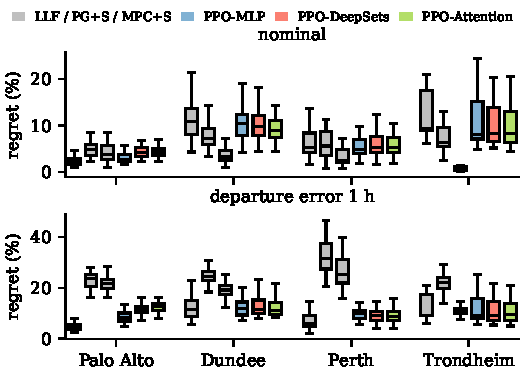
\includegraphics[width=\columnwidth]{fig_regret.pdf}
\caption{Distribution of the weekly regret on held-out sites (E2). Grey boxes, from left to right:
LLF, price-greedy+S and MPC+S. PPO boxes use the seed-averaged regret of each week.}
\label{fig:regret}
\end{figure}

The components of the objective explain these positions (site averages). Under nominal conditions, MPC+S paid 0.966 times the mean
price per delivered kWh and delivered 97.2\% of the requested energy, LLF paid 1.034 and delivered
98.9\%, and ASAP paid 1.034 and delivered 96.6\%. The PPO agents delivered 98.2--98.5\% at
1.018--1.023: a delivered fraction near that of LLF and a smaller part of the price reduction obtained
by MPC.

\subsection{Errors in the announced departure}
When the announced departures were perturbed by $\mathcal N(0,1\,\mathrm h)$, the mean regret of
MPC+S rose from 3.6\% to 21.6\% and that of price-greedy+S from 6.4\% to 26.1\%, while LLF rose from
7.6\% to 8.9\% and the PPO agents from 7.1--7.5\% to 10.9--11.9\% (Table~\ref{tab:main}). The
delivered fraction fell to 88.1\% for MPC+S and 86.9\% for price-greedy+S, against 95.6--96.5\% for
PPO and 98.2\% for LLF: a plan that finishes each vehicle at its announced departure leaves energy
undelivered whenever the vehicle leaves earlier.
All three PPO encoders had a lower regret than MPC+S at Palo Alto, Dundee and Perth
($p_\mathrm{Holm}<10^{-4}$), with no difference detected at Trondheim ($p_\mathrm{Holm}\ge0.52$). Compared
with LLF, PPO had a higher regret at Palo Alto and Perth ($p_\mathrm{Holm}<10^{-7}$), no difference
detected at Dundee ($p_\mathrm{Holm}\ge0.30$) and a lower regret at Trondheim ($p_\mathrm{Holm}\le0.01$).
Lee et al. found user-provided departures to be the least accurate of the estimators compared on
ACN-Data~\cite{lee2019acndata}, so an MPC that uses them inherits their error; Li and Sun make the
same distinction between a data-independent MPC and an RL policy shaped by its training
data~\cite{li2023ood}. Here the PPO agents were trained with departure-noise
randomization~\cite{tobin2017domain}, whose contribution is isolated in the ablation below.

\subsection{Encoders and transfer gap}
Differences between encoders depended on the site. At Palo Alto, the site with the shortest dwell
times (Table~\ref{tab:data}), the flat MLP had a lower regret than both set encoders (median
difference 1.0--1.1 points, $p_\mathrm{Holm}<10^{-8}$); at Trondheim, the residential site, the
attention encoder had a lower regret than the MLP (10.8\% vs 12.4\%, $p_\mathrm{Holm}=0.012$).
Trondheim, with 12 test weeks, also had the largest standard deviation over seeds (1.6--2.4 points),
the seed dependence that Henderson et al. reported for DRL~\cite{henderson2018matters}. Within the
E2 runs, each site is a training source in three of the four configurations, which gives a
transfer gap in the sense of the difference between training and test
performance~\cite{kirk2023survey}: the regret on a site when it was held out minus the regret on the same
site when it was a source averaged 0.5 (DeepSets), 0.6 (attention) and 0.8 (MLP) points, with the
largest gap at Dundee (1.5--2.4 points).

Fig.~\ref{fig:transfer} reports the single-source experiment (E1, two seeds). For DeepSets, the mean
regret on the diagonal (trained and tested on the same site) was 6.1\% and off the diagonal 7.5\%;
for the MLP, 5.5\% and 5.8\%. Training on Palo Alto, the site with the shortest dwell times, gave the
highest regrets on Dundee and Trondheim for both encoders (DeepSets 13.1\% and 14.6\%). For Trondheim,
the best single source (MLP trained on Perth, 7.8\%; DeepSets trained on Dundee, 9.0\%) had a lower
regret than the corresponding E2 agents trained on three sources (12.4\% and 11.3\%), so pooling
sources did not by itself reduce the regret at the held-out site.
\begin{figure}[t]
\centering
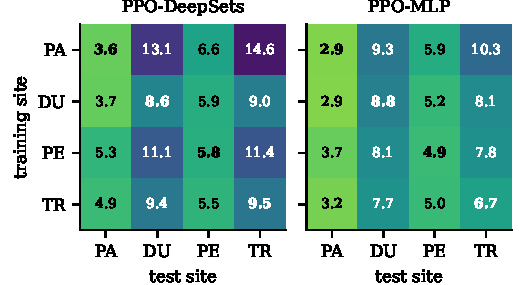
\includegraphics[width=\columnwidth]{fig_transfer.pdf}
\caption{Single-source transfer (E1): mean regret (\%) on the test weeks of each site (columns) for
agents trained on one site (rows), two seeds; diagonal in bold.}
\label{fig:transfer}
\end{figure}

\subsection{Ablations (E3)}
Table~\ref{tab:abl} compares the DeepSets agent (seed 0) with four variants, each removing one element
of the training design, over the 143 test weeks of the held-out sites (paired Wilcoxon tests against
the full configuration). The nominal regret rose without the centred price ($p=3\times10^{-10}$; at
Trondheim from 10.3\% to 23.5\%), without shaping ($p=6\times10^{-8}$) and with one action per slot
($p=9\times10^{-6}$). Training without departure noise lowered the nominal regret (median difference
$-0.34$ points, $p=0.014$) and raised the regret under departure error ($p=9\times10^{-17}$), the
trade-off that domain randomization targets~\cite{tobin2017domain}.

\begin{table}[t]
\caption{Ablations (E3): DeepSets, leave-one-site-out, seed 0; mean over the four held-out sites.
Delivered energy and cost are under nominal conditions.}
\label{tab:abl}
\centering
\footnotesize
\setlength{\tabcolsep}{3pt}
\begin{tabular}{lcccc}
\toprule
 & \multicolumn{2}{c}{Regret (\%)} & Delivered & Cost\\
Variant & Nominal & Dep. error & (\%) & \\
\midrule
Full configuration & 7.2 & 11.4 & 98.2 & 1.019\\
No centred price & 10.0 & 19.7 & 96.9 & 1.021\\
No shaping & 7.6 & 12.2 & 98.2 & 1.022\\
One action per slot & 7.8 & 17.2 & 98.1 & 1.022\\
No departure noise in training & 6.3 & 17.0 & 97.7 & 1.001\\
\bottomrule
\end{tabular}
\end{table}

\subsection{Example week and computation time}
Fig.~\ref{fig:week} shows the first four days of a Dundee test week (Dundee held out). MPC+S
concentrated charging in the low-price hours, alternating between zero and $\bar P$; LLF charged at
$\bar P$ whenever vehicles were present; PPO-DeepSets lowered the set-point in high-price hours while the
urgent rates kept charging active. Over this week, the energy cost per delivered kWh was 1.038 (LLF),
0.955 (MPC+S) and 1.018 (PPO), and the delivered fraction 99.8\%, 98.6\% and 99.7\%.
On one CPU thread (\texttt{scripts/timing.py}), a PPO decision including the safety layer took
0.6--0.9\,ms (MLP), 1.1--1.7\,ms (DeepSets) and 1.4--1.8\,ms (attention), an MPC+S step 0.9--2.6\,ms on
average (maxima 13--31\,ms) and an LLF step 0.03\,ms, for a 15-min control interval.

For a charge point operator with a contracted power limit, two cases follow from these results. Where
drivers announce departures through an app without incentives to be accurate~\cite{lee2019acndata},
MPC+S left 11.9\% of the energy undelivered in the departure-error test, the PPO agents 3.5--4.4\% and
LLF 1.8\%. Where departures are known, as in a fleet depot with fixed shifts, MPC+S had the lowest
regret at three of the four sites.

\begin{figure}[t]
\centering
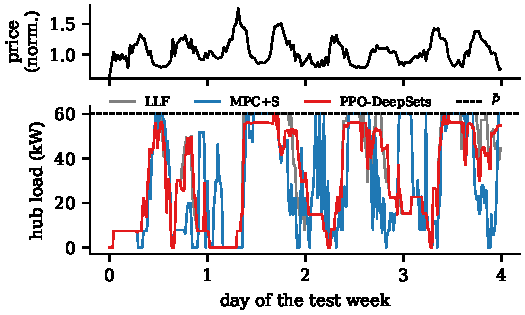
\includegraphics[width=0.76\columnwidth]{fig_week.pdf}
\caption{Price and hub load, Dundee test week, Dundee held out (PPO-DeepSets, seed 0).}
\label{fig:week}
\end{figure}

%=========================================================================================
\section{Conclusion}
%=========================================================================================
Trained on three sites and tested on the fourth, the PPO controller had a mean regret 0.1--0.5 points
below LLF and 3.5--3.9 points above MPC under nominal conditions, and 2.0--3.1 points above LLF and
9.6--10.7 points below MPC with a 1\,h departure error. The encoder with the lowest regret depended on
the site, and the transfer gap averaged 0.5--0.8 points. The choice between optimization and a learned
policy therefore depends on how reliable the announced departures are~\cite{lee2019acndata}.

Limitations: one GB price series was used for all sites; each dataset was treated as one
virtual hub with a single limit, without the unbalanced three-phase infrastructure, non-ideal
battery behaviour and quantized control signals described for the ACN~\cite{lee2021acn}; the delivered energy was taken as the
requested energy and the departure error was synthetic; the hub limit and $\lambda$ were fixed; the
attention encoder was not tuned; E1 and E3 used two and one seeds; training was limited to
$1.5\times10^6$ steps on a laptop CPU. Future work includes site-specific
prices, per-location hubs with three-phase limits as in ACN-Sim~\cite{lee2021acnsim}, MPC with arrival
forecasts, policies that combine a learned component with the optimization plan, vehicle-to-grid
operation~\cite{orfanoudakis2025ev2gym}, and a field evaluation. The datasets are
public~\cite{paloalto,dundee,perth,sorensen2021data,elexon}; the code that produces every table and
figure of this paper is available at \url{https://github.com/GabyQueiroz/ICIT2027-EVRL}.

\textit{Declaration of generative AI use:} Claude (Anthropic) assisted in writing the code, running the experiments and drafting the text; the
authors reviewed all of it and take responsibility for the content.

\bibliographystyle{IEEEtran}
\bibliography{refs}

\end{document}
